\documentclass[12pt, a4paper, oneside]{article} 
% velikost písma, stránky, typ dokumentu -- detaily viz literatura

%\usepackage{c} % nastavení češtiny
%\usepackage[latin2]{inputenc}
%\usepackage[cp1250]{inputenc} % pro win1250
\usepackage[center]{caption} 
\usepackage[utf8]{inputenc}
\usepackage{wrapfig} % nastavení obtékání textu
\usepackage{graphicx,amsmath} % nastavení grafiky, matematiky
\usepackage{subfig} % více obrázků vedle sebe 
\usepackage{float}
\usepackage{amsmath}
\usepackage{amssymb}
\usepackage{bbding}
\usepackage{enumitem}
\usepackage{breakurl}
\usepackage{pdflscape}
\usepackage{wrapfig}

%\usepackage{indentfirst}

\usepackage{tocloft} %přidá tečky do obsahu ke kapitolám /sekcím 
\renewcommand{\cftsecdotsep}{\cftdotsep}

\usepackage[bookmarksopen,colorlinks,plainpages=false,linkcolor=black,urlcolor=blue,citecolor=black,filecolor=black,menucolor=black,unicode=true]{hyperref}

\urlstyle{rm}
%bookmarksopen -- open up bookmark tree 
%colorlinks -- zbarví odkazy (implicitně orámovaný nezbarvený text)
%urlcolor -- barva odkazů (implicitně magenta) 
%linkcolor=black -- barva odkazů v obsahu (implicitně red)

\usepackage{listings}
\usepackage{color}
\usepackage{minted}
\definecolor{lightgray}{RGB}{240,240,240}
\definecolor{darkgray}{rgb}{.4,.4,.4}
\definecolor{purple}{rgb}{0.65, 0.12, 0.82}
\definecolor{darkgreen}{RGB}{0,150,0}

\usemintedstyle{perldoc}
\newminted{js}{linenos=true, bgcolor=lightgray}

\lstdefinelanguage{JavaScript}{
  keywords={typeof, new, true, false, catch, function, return, null, catch, switch, var, if, in, while, do, else, case, break, for},
  keywordstyle=\color{blue}\bfseries,
  ndkeywords={class, export, boolean, throw, implements, import, this},
  ndkeywordstyle=\color{blue}\bfseries,
  identifierstyle=\color{black},
  sensitive=zr,
  comment=[l]{//},
  morecomment=[s]{/*}{*/},
  commentstyle=\color{darkgreen}\ttfamily,
  stringstyle=\color{red}\ttfamily,
  morestring=[b]',
  morestring=[b]"
}

\lstset{
   backgroundcolor=\color{lightgray},
   extendedchars=true,
   basicstyle=\footnotesize\ttfamily,
   showstringspaces=false,
   showspaces=false,
   numbers=left,
   numberstyle=\footnotesize,
   numbersep=9pt,
   tabsize=2,
   breaklines=true,
   showtabs=false,
   aboveskip=5mm,
   belowskip=7mm,
   captionpos=b
}

\renewcommand{\listingscaption}{Code sample}
\renewcommand{\listoflistingscaption}{Code samples}

% \usepackage{parskip} -- zapne americké odstavce v celé práci

\addtolength{\textwidth}{25mm}
\addtolength{\hoffset}{-12.5mm}
\addtolength{\textheight}{35mm}

\setlength{\intextsep}{5mm} % nastavení mezery okolo obrázků

% nastavení příkazu >\figcaption pro popis čehokoli, jako by to byly obrázky 
\makeatletter   
\newcommand\figcaption{\def\@captype{figure}\caption}
\makeatother

\renewcommand\refname{Literatura} 
%\def\bibname{PŘÍLOHA D: Reference}
%\renewcommand\bibname{PŘÍLOHA D: Reference}
% přejmenuje anglický název Reference na české Literatura


%\makeindex % příprava pro výrobu indexu (jestli ho chcete)

%%    VLNKA <fileinput>  KkSsVvZzOoUuAaIi        
% Defaultni  koncovka pro <fileinput> je  ".tex"
%FIXME: haze error
%\cstieon % Vypne chovani vlnky jako tvrde mezery v matematickem rezimu

%%%%%%%%%%%%%%%%%%%%%%%%%%%%%%%%%%%%%%%%%%%%%%%%%%%%%%%%%%%%%%%
%V PROSTŘEDÍ ROVNIC SE NESMÍ VYSKYTOVAT PRÁZDNÝ ŘÁDEK
%
%PROGRAMY VLNKA A CSINDEX SE MUSÍ SPUSTIT SAMOSTATNĚ
%%%%%%%%%%%%%%%%%%%%%%%%%%%%%%%%%%%%%%%%%%%%%%%%%%%%%%%%%%%%%%%

% definice příkazů 
\newcommand{\D}{\medskip \noindent} % nový odstavec v "americkém" formátování 
\newcommand{\B}{\textbf} %tučné písmo
\newcommand{\A}{\mathbf} %tučné písmo v matematickém režimu
\newcommand{\TO}{\ensuremath{\boldsymbol\Omega}} % tučný znak velké omega -- pro ohmy
\newcommand{\I}{\index}  % vytváří položku indexu (asi nepoužijete)
\newcommand{\Deg}[1][]{\ensuremath{{#1}^\circ}} % vysází značku stupně Celsia
\newcommand{\Def}{\footnotesize Definice: \normalsize}
\newcommand{\Pos}{\footnotesize Experiment: \normalsize}
\newcommand{\Odv}{\footnotesize Odvození: \normalsize}
\newcommand{\Vym}{\footnotesize Vymezení pojmu: \normalsize}
\newcommand{\Ob}{obrázek }
\newcommand{\It}{\textit}  % kurzíva
\newcommand{\M}{\mathrm}   % v prostředí rovnic nastaví normální písmo (místo kurzívy ) 
\newcommand{\F}{\footnotesize} % zmenšená velikost písma
\newcommand{\N}{\normalsize} % normální velikost písma
%\newcommand{\U}{\underline}  % podtržené písmo
\newcommand{\e}{\ensuremath} 
\newcommand{\Has}{\textcolor{green}{\CheckmarkBold}}
\newcommand{\NoHas}{\textcolor{red}{\XSolidBrush}}
% další příkaz se aplikuje, pouze, když jste v matematickém režimu

%\hyphenation{Pusť-me pla-tí hod-no-ty do-sa-dí-me za-da-né dal-ším}
% dělení slov, kdyby implicitní nevyhovovalo

\linespread{1.1}
% řádkování 1,5x  
% použijete podle situace  

\unitlength=1mm % nastavení volby jednotek 

% www.amavet.cz www.fvtp.cz

% titulek - přidat školu a zemi - přeložit - loga pryc
% abstrakt - kontaktní údaje, web, email - spojit adresu

% konec hlavičky
%%%%%%%%%%%%%%%%%%%%%%%%%%%%%%%%%%%%%%%%%%%%%%%%%%%%%%%%%%%%%%%%%%%
%%%%%%%%%%%%%%%%%%%%%%%%%%%%%%%%%%%%%%%%%%%%%%%%%%%%%%%%%%%%%%%%%%%

\pagestyle{empty}

\begin{document}
\setlength{\voffset}{-20mm}
\begin{center}

\Large
\B{LORRIS TOOLBOX} \\
\large
\B{Microprocessor Application Development Kit}
\url{http://tasssadar.github.io/Lorris}

\end{center}

\begin{figure}[H]
\begin{center}
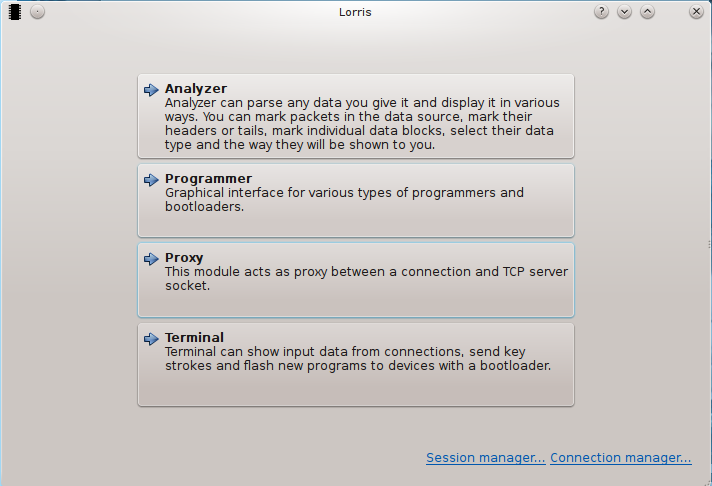
\includegraphics[scale=0.6]{../img/new_tab.png}
\caption{Tab creation dialog}
\end{center}
\end{figure}

\begin{figure}[H]
\begin{center}
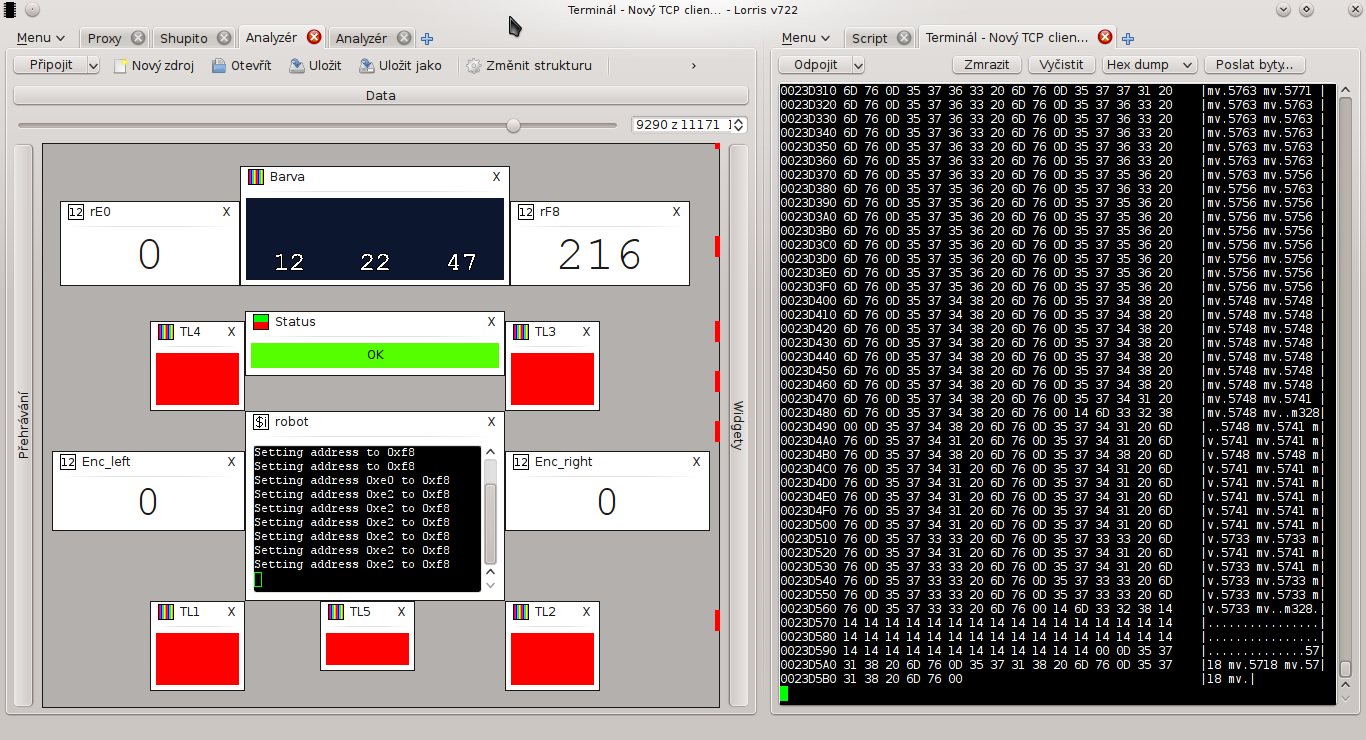
\includegraphics[width=\textwidth]{../img/split.png}
\caption{Lorris' window divided to multiple parts}
\end{center}
\end{figure}

\begin{figure}[h]
\begin{center}
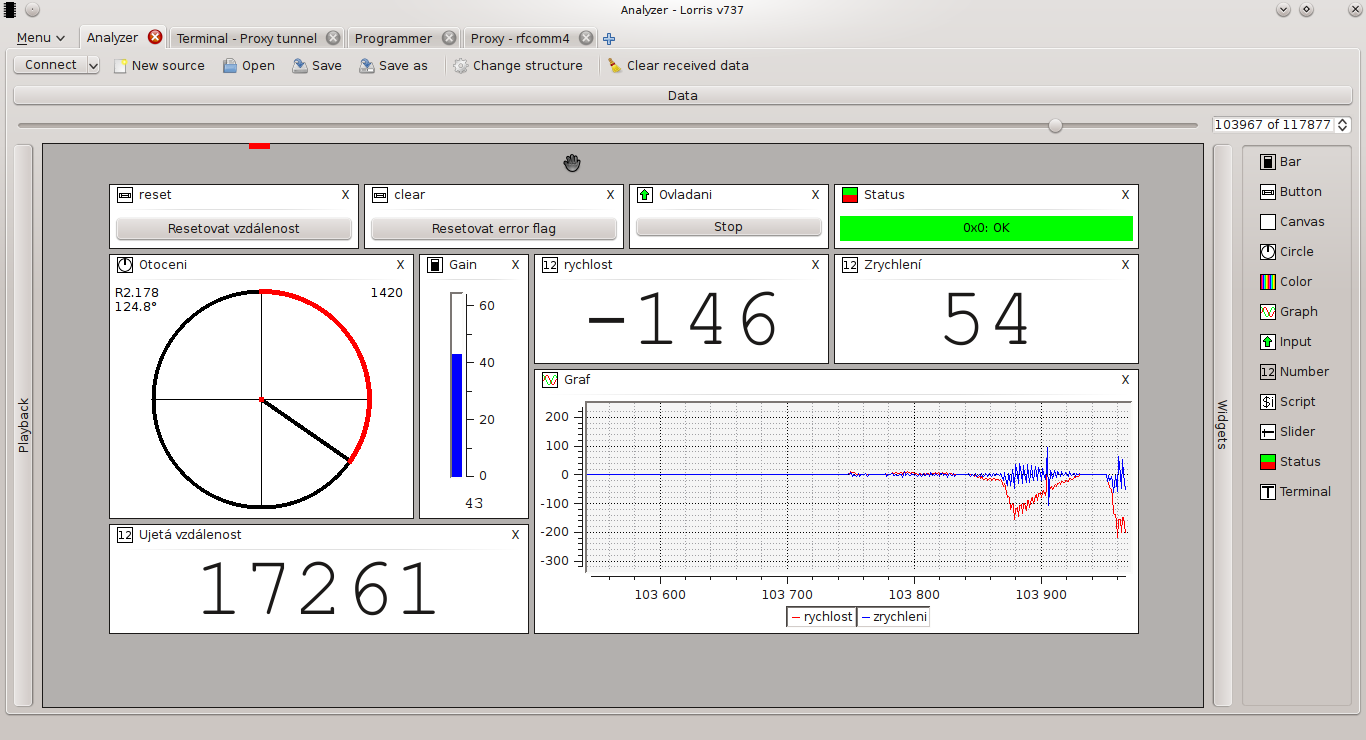
\includegraphics[width=\textwidth]{../img/analyzer_all.png}
\caption{\B{Analyzer} module}
\end{center}
\end{figure}

\begin{figure}[H]
\begin{center}
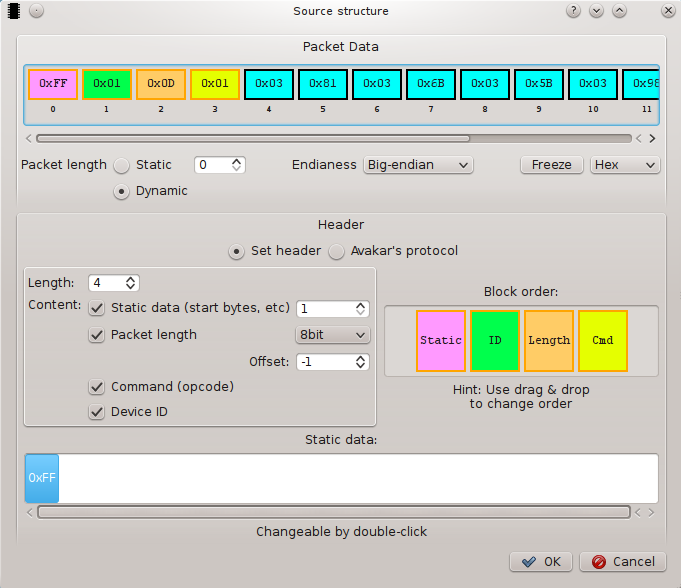
\includegraphics[scale=0.75]{../img/analyzer_struct.png}
\caption{\B{Analyzer:} packet structure dialog}
\label{Analyzer_struct}
\end{center}
\end{figure}

\begin{figure}[H]
\begin{center}
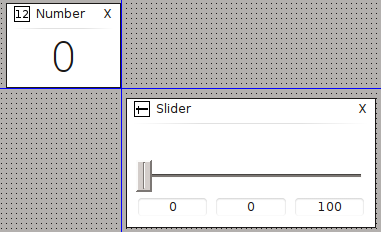
\includegraphics[scale=1]{../img/lines.png}
\caption{\B{Analyzer:} widget aligment using grid and lines}
\label{widget_lines}
\end{center}
\end{figure}

\begin{figure}[H]
\begin{center}
\subfloat[List of widgets]{\label{analyzer_widgets}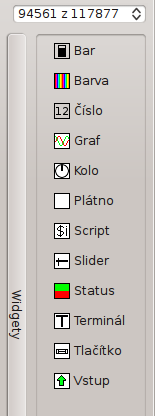
\includegraphics[scale=1]{../img/analyzer_widgets_new.png}}
\hfill
\subfloat[Assigning data using drag\&drop]{\label{analyzer_widgets}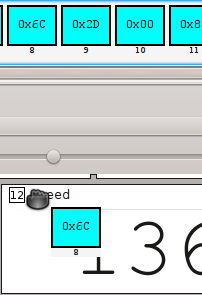
\includegraphics[scale=1]{../img/analyzer_drag_data.png}}  
\caption{\B{Analyzer:} widgets}
\label{widgets}
\end{center}
\end{figure}

\begin{figure}[H]
\begin{center}
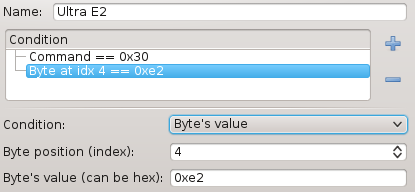
\includegraphics[scale=0.9]{../img/filters.png}
\caption{\B{Analyzer:} data filter settings}
\end{center}
\end{figure}

\begin{listing}[H]
\begin{jscode}
// Return true if passes, false if it
// should be filtered out
function dataPass(data, dev, cmd) {
    return false;
}
\end{jscode}
\caption{\B{Analyzer:} data filter script condition}
\end{listing}

\begin{figure}[h]
\begin{center}
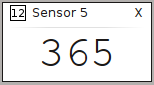
\includegraphics[scale=1]{../img/w_num.png}
\caption{\B{Analyzer:} widget number}
\end{center}
\end{figure}

\begin{figure}[H]
\begin{center}
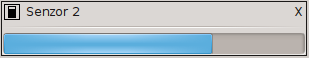
\includegraphics{../img/w_bar.png}
\caption{\B{Analyzer:} widget bar}
\end{center}
\end{figure}

\begin{figure}[H]
\begin{center}
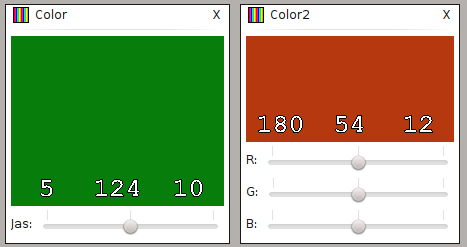
\includegraphics{../img/w_col.png}
\caption{\B{Analyzer:} widget color}
\end{center}
\end{figure}

\begin{figure}[h]
\begin{center}
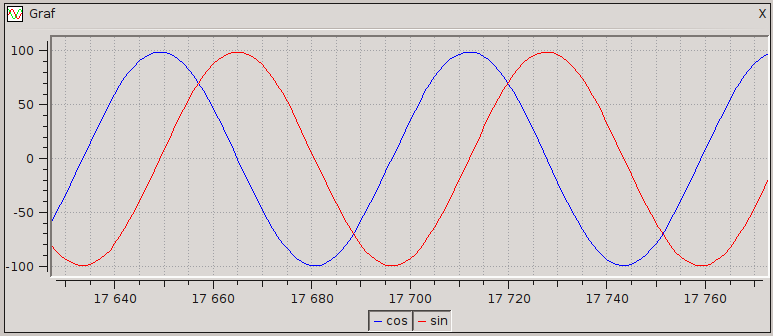
\includegraphics[scale=0.7]{../img/w_graph.png}
\caption{\B{Analyzer:} widget graph}
\end{center}
\end{figure}

\begin{figure}[h]
\begin{center}
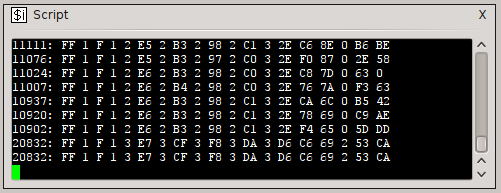
\includegraphics[scale=1.0]{../img/w_script.png}
\caption{\B{Analyzer:} widget script}
\label{script_w}
\end{center}
\end{figure}

\begin{figure}[h]
\begin{center}
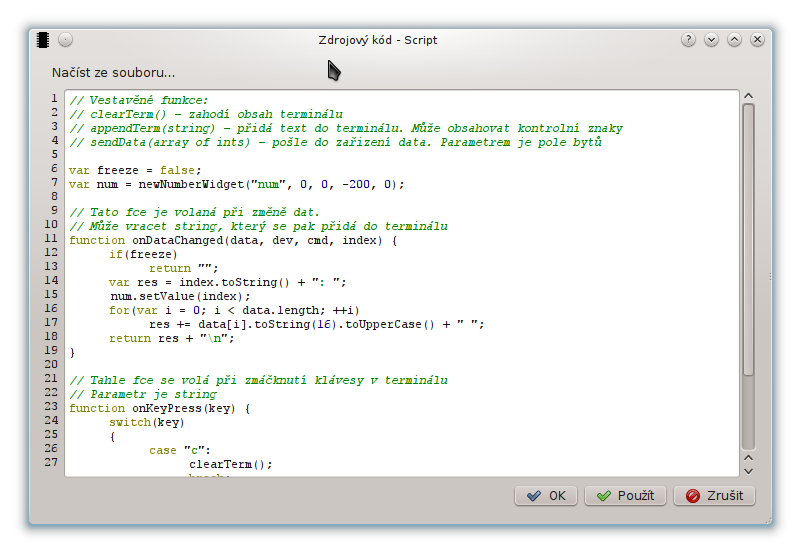
\includegraphics[width=\textwidth]{../img/w_script_src.png}
\caption{\B{Analyzer:} widget script: editor}
\label{script_src}
\end{center}
\end{figure}

\begin{figure}[H]
\begin{center}
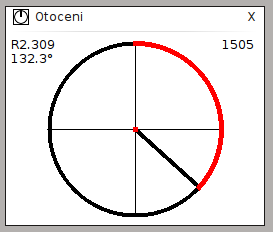
\includegraphics[scale=1]{../img/w_circle.png}
\caption{\B{Analyzer:} widget circle}
\end{center}
\end{figure}

\begin{figure}[H]
\begin{center}
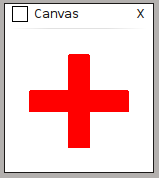
\includegraphics[scale=1]{../img/w_canvas.png}
\caption{\B{Analyzer:} widget canvas}
\end{center}
\end{figure}

\begin{listing}[H]
\begin{jscode}
Canvas.setLineColor("red");
Canvas.setFillColor("red");
// x, y, width, height
Canvas.drawRect(55, 10, 20, 110);
Canvas.drawRect(10, 55, 110, 20);
\end{jscode}
\caption{\B{Analyzer:} widget canvas: drawing to widget from script}
\end{listing}

\begin{figure}[H]
\begin{center}
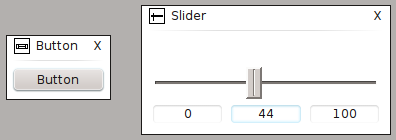
\includegraphics[scale=1]{../img/w_btn_slider.png}
\caption{\B{Analyzer:} widgets button and slider}
\end{center}
\end{figure}

\begin{listing}[H]
\begin{jscode}
function Slider_valueChanged() {
    appendTerm("Slider value: " + Slider.getValue() + "\n");
}

function Button_clicked() {
    appendTerm("Button clicked\n");
}
\end{jscode}
\caption{\B{Analyzer:} widget \It{slider} and \It{button} callbacks in script}
\end{listing}

\begin{figure}[H]
\begin{center}
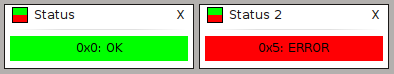
\includegraphics[scale=1]{../img/w_status.png}
\caption{\B{Analyzer:} widget status}
\end{center}
\end{figure}

\begin{figure}[H]
\begin{center}
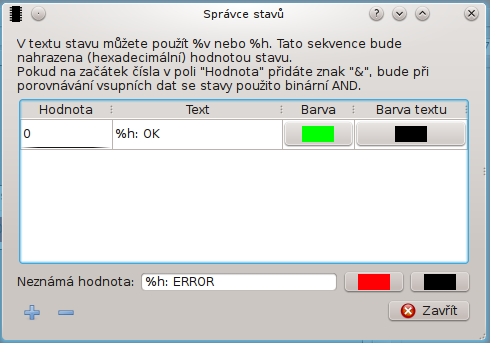
\includegraphics[scale=0.7]{../img/w_status_dlg.png}
\caption{\B{Analyzer:} widget status: state definitions dialog}
\label{status_dlg}
\end{center}
\end{figure}

\begin{figure}[H]
\begin{center}
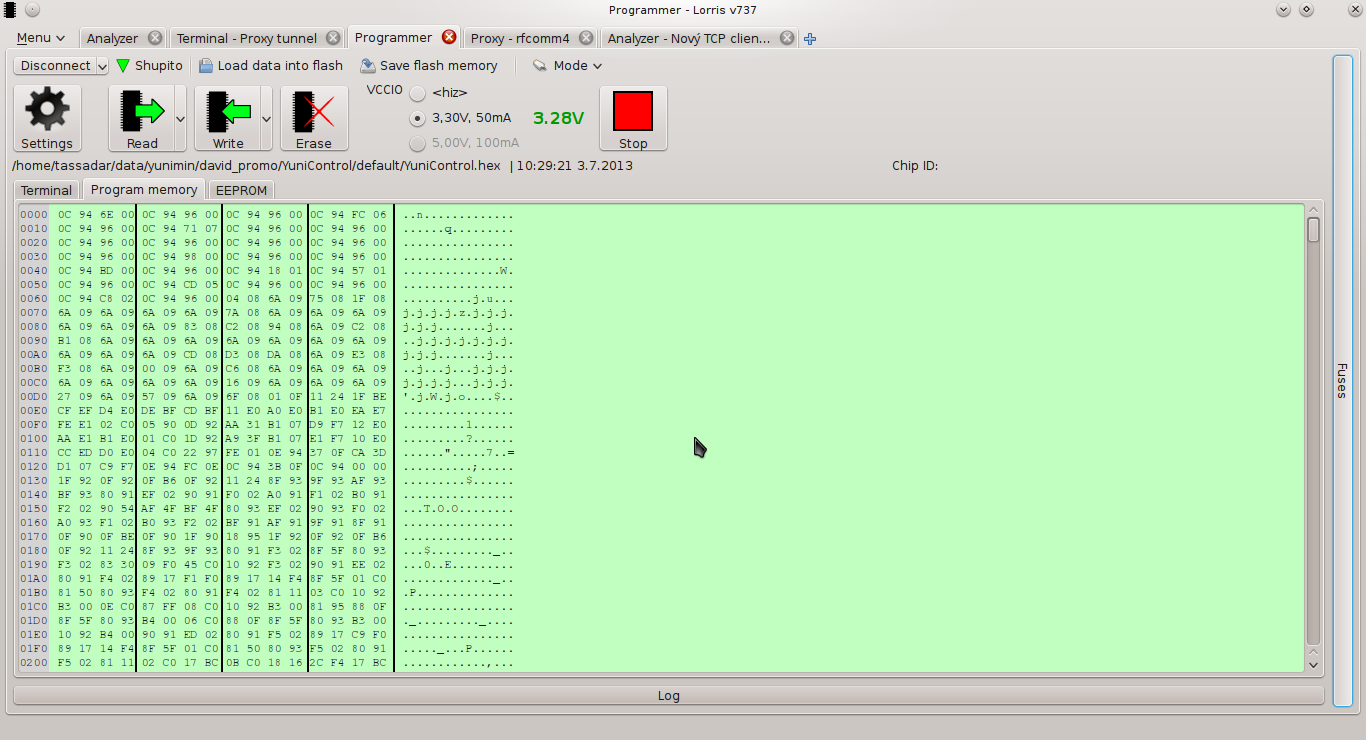
\includegraphics[width=\textwidth]{../img/programmer.png}
\caption{\B{Programmer} module}
\label{prog_full}
\end{center}
\end{figure}

\begin{figure}[H]
\begin{center}
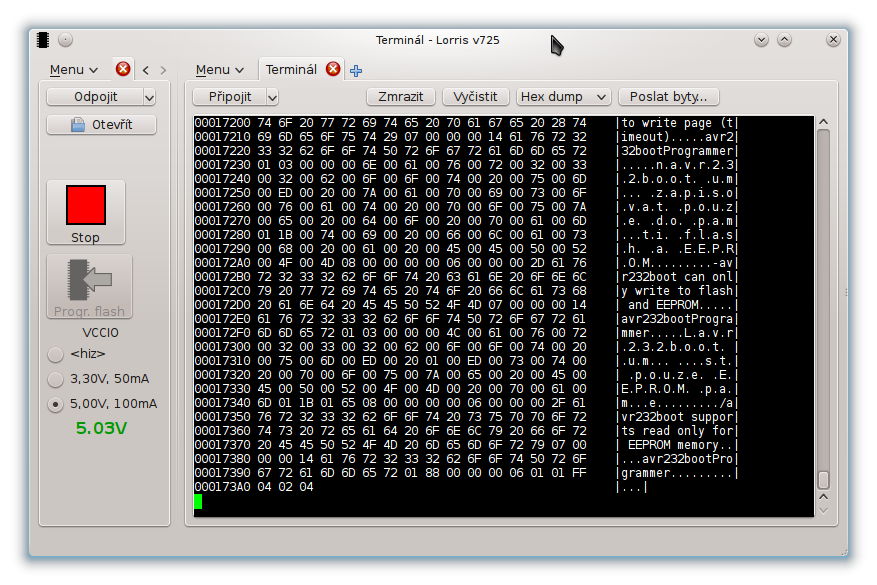
\includegraphics[width=\textwidth-30pt]{../img/programmer_mini.png}
\caption{\B{Programmer:} minimal interface (left) along with \It{terminal} (right)}
\label{prog_mini}
\end{center}
\end{figure}

\begin{figure}[H]
\begin{center}
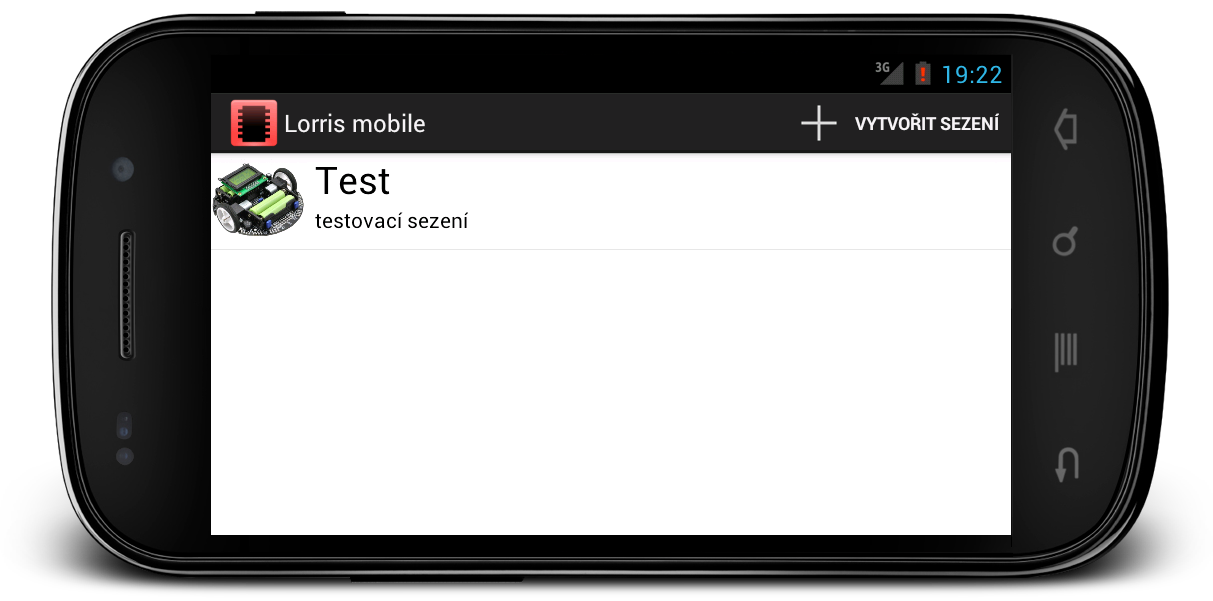
\includegraphics[width=\textwidth]{../img/mobile_session.png}
\caption{\B{Lorris mobile:} session selection}
\label{mobile_session}
\end{center}
\end{figure}

\begin{figure}[H]
\begin{center}
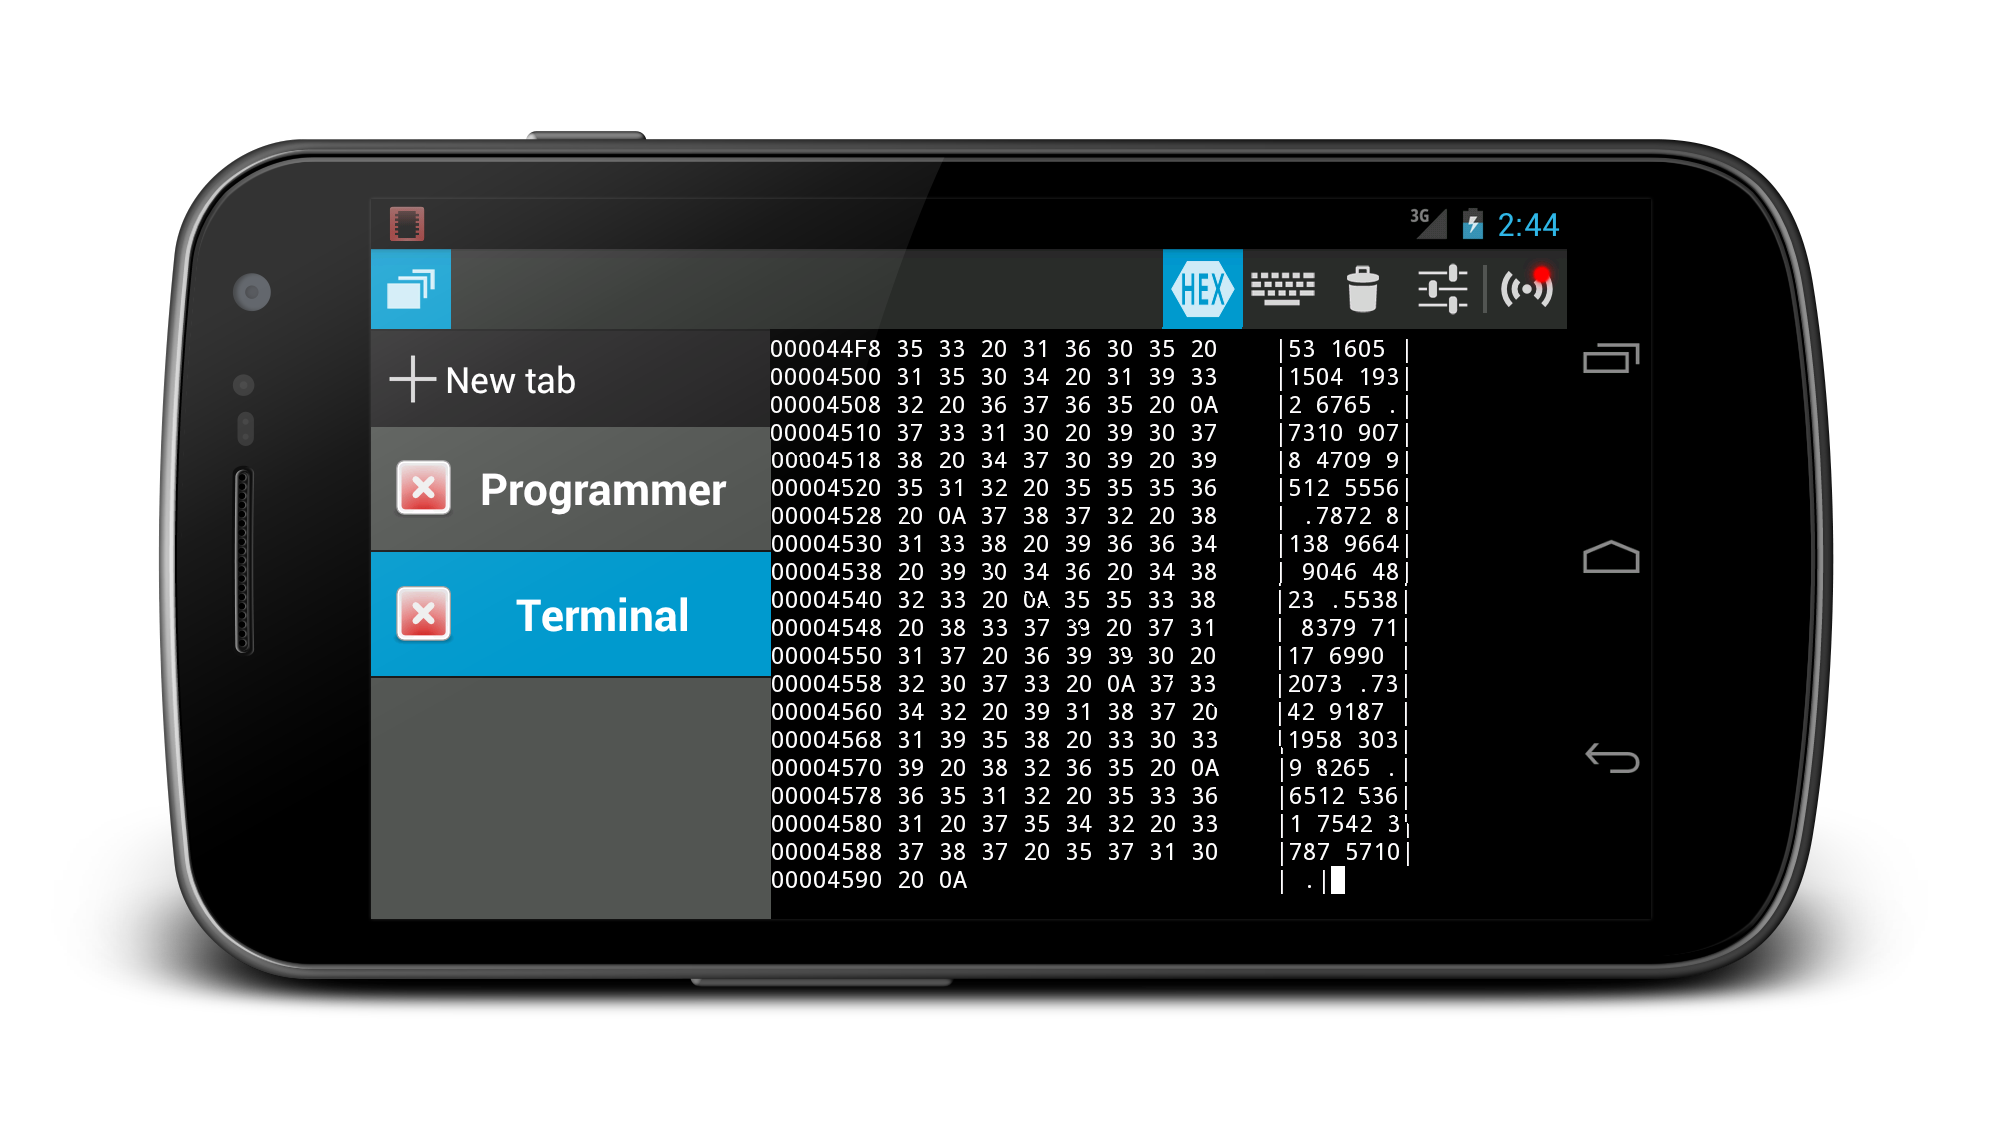
\includegraphics[width=\textwidth]{../img/mobile.png}
\caption{\B{Lorris mobile}: terminal}
\end{center}
\end{figure}

\begin{figure}[H]
\begin{center}
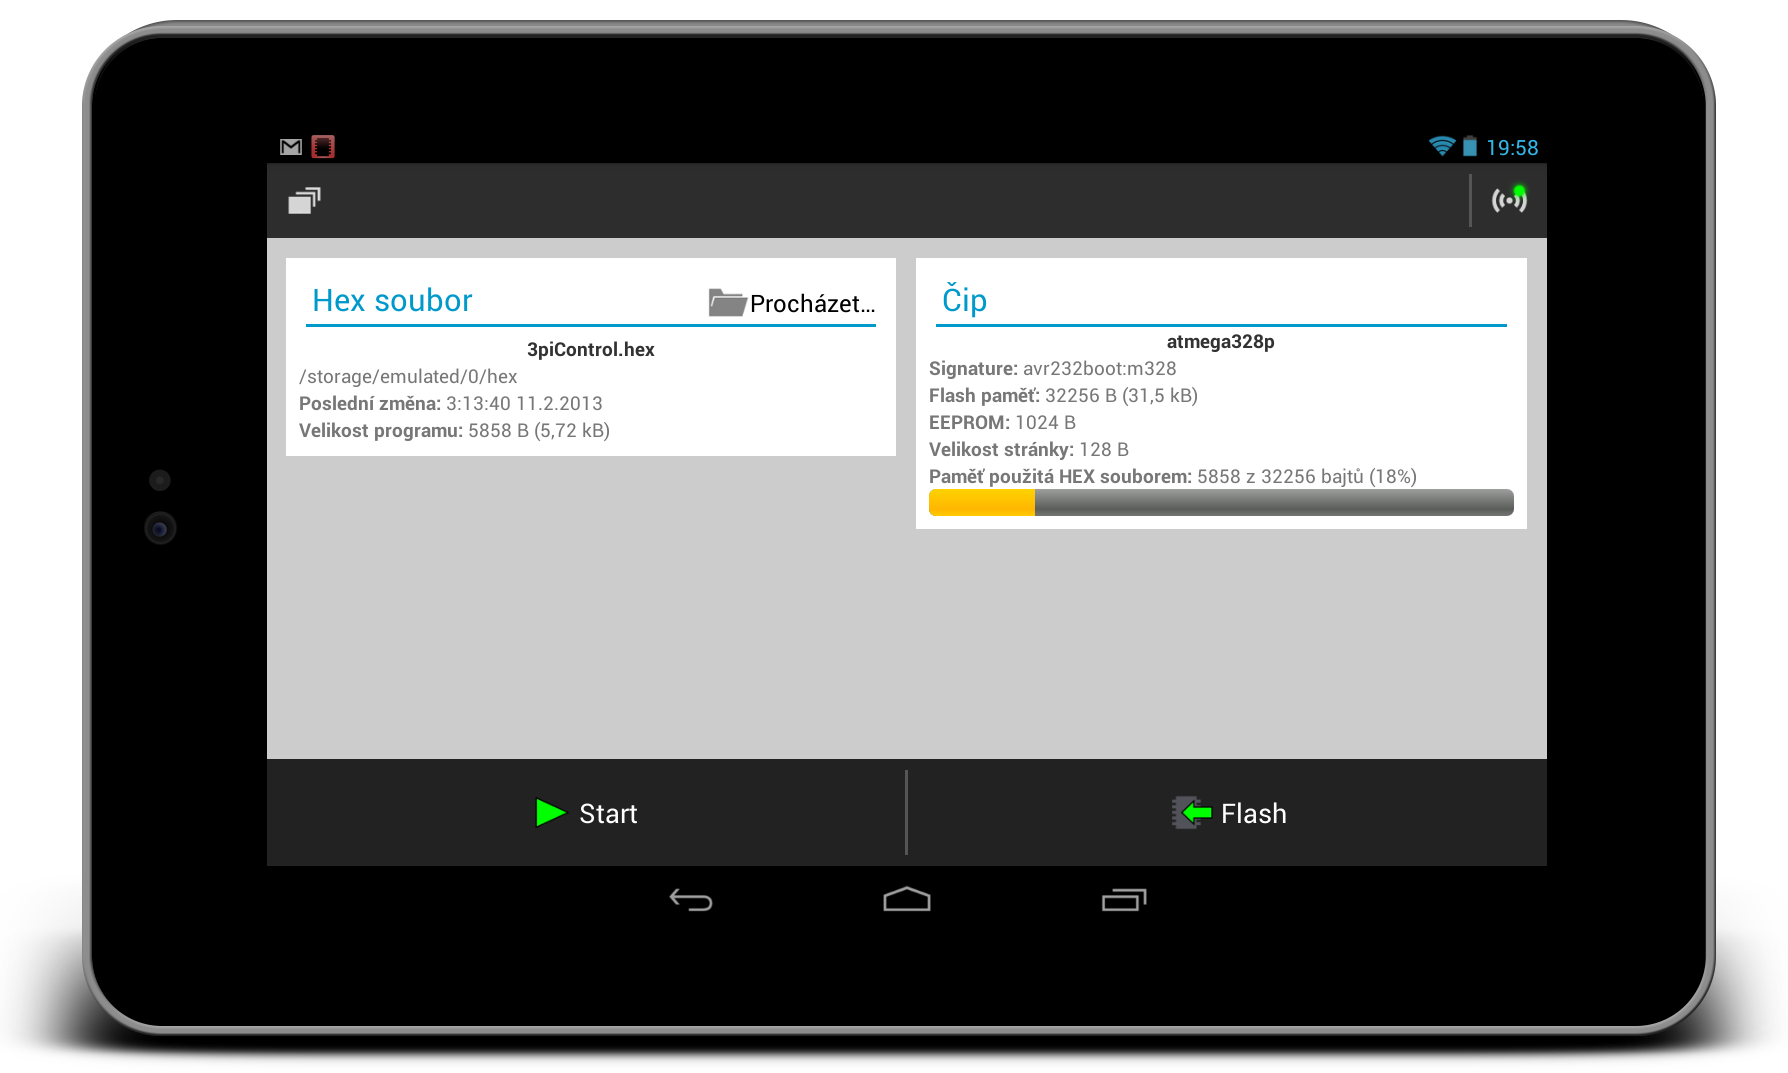
\includegraphics[width=\textwidth]{../img/mobile_programmer.png}
\caption{\B{Lorris mobile:} programmer}
\end{center}
\end{figure}

\end{document}
